\documentclass[11pt]{article}
\usepackage{amsmath,amssymb,color,hyperref,graphicx,pdfsync}
\usepackage{svn}
\SVN $Date$
\SVN $Revision$
\SVN $Author$
\SVN $HeadURL$
\newcommand\revisioninfo{\centerline{\textcolor{blue}{Revision: \SVNRevision ; Last changed by \SVNAuthor\ on \SVNDate .}}}

\graphicspath{{Figures/}}

\textwidth 5.5 truein
\oddsidemargin .5 truein
\evensidemargin .5 truein
\topmargin -.5 truein
\textheight 8.5in

\def\todo#1{\textcolor{blue}{{\bf To do:} #1}}
\def\question#1{\textcolor{red}{\bf Question:} #1}

%\def\code#1{{\ttfamily #1}}
\def\class#1{{\bf #1}} % \bfseries
\def\fn#1{{\tt #1}} % \ttfamily
\def\virtualfn#1{{\it #1}} % \itshape

\def\cmd#1{{\bfseries #1}}
\def\ttcmd#1{{\ttfamily\cmd{#1}}}
\def\arg#1{\textit{#1}}
\def\optarg#1{[\arg{#1}]}
% \def\<#1>{\leavevmode\hbox{$\langle$#1\/$\rangle$}} % syntactic quantity
% \def\[#1]{\leavevmode\hbox{$\langle$#1\/$\rangle$}} % optional argument
% \def\spc{\<\small SPACE>}
% \def\return{\textit{Return}}
% \def\control{\textit{Control}}
% \def\meta{\textit{Meta}}
% \def\esc{{\small ESC}}

% % for verbatim entries (from Knuth's manmac)
% \chardef\other=12
% \def\ttverbatim{\begingroup \catcode`\\=\other \catcode`\{=\other
%   \catcode`\}=\other \catcode`\$=\other \catcode`\&=\other
%   \catcode`\#=\other \catcode`\%=\other \catcode`\~=\other
%   \catcode`\_=\other \catcode`\^=\other
%   \obeyspaces \obeylines \tt}
% \newskip\ttglue
% \ttglue=.5em plus.25em minus.15em
% {\catcode`\|=\active \obeylines
% \gdef|{\ttverbatim\spaceskip=\ttglue\let^^M=\ \let|=\endgroup}}
% \catcode`\|=\active

% % for command line displays (from Knuth's manmac)
% \outer\def\begintt{$$\let\par=\endgraf \ttverbatim \parskip=0pt
%   \catcode`\|=0 \rightskip=-5pc \ttfinish}
% {\catcode`\|=0 |catcode`|\=\other % | is temporary escape character
%   |obeylines % end of line is active
%   |gdef|ttfinish#1^^M#2\endtt{#1|vbox{#2}|endgroup$$}}

\begin{document}

\title{Design document for Immersed Boundary Projection Method (IBPM)}
\author{Clancy Rowley}
\date{\revisioninfo}
\maketitle

\section{Purpose of this document}
This document describes the design of a code to implement the fast (multiple-grid) Immersed Boundary Projection Method (IBPM) of Colonius and Taira \cite{ColTai-07}.  Here we give a high-level overview of the classes planned, interactions between them, and their public interfaces.  Where appropriate, we describe ideas for possible implementations, but for the most part we leave implementation to the detailed class design.

The design here addresses only the single-grid case, rather than the more complex multiple-grid case.  The philosophy here was that we will probably want to iterate and refine this design, and will learn along the way (for instance, when implementing the boundary conditions and learning more about the dependencies), so it probably does not make sense to design for multiple grids at the outset.

This document is not intended to be a ``living'' document that evolves as changes are made to the code, and thus should not be taken as the definitive documentation.  The intent is for the ``living'' documentation to be contained within the code itself, to be extracted using Doxygen, and for this document to serve both as a blueprint for construction, and as a reference for how and why design decisions were made.  If major changes to the structure are made, however (such as extending to the multiple-grid case), then it would be appropriate to revise this document, or write a new one.

\tableofcontents

\section{History and design approach}

\subsection{Previously used code and its limitations}
Prior to the development of the code described in this document, we have been using an implementation of the Immersed Boundary Projection Method (IBPM) written by Colonius and Taira, using Fortran 90.  However, because of the complexity and the tight coupling of the Fortran implementation, this code has become difficult to maintain.  For instance, we wished to change the timestepper, from a second-order Adams-Bashforth/Crank-Nicolson scheme (a two-step scheme) to a Runge-Kutta/Crank-Nicolson scheme, both for improved timestep restrictions, and to sidestep certain issues with a multi-step scheme, when used for adjoint simulations, eigenvalue solvers, and the like.  However, the Fortran~90 code is tightly coupled, making extensive use of global or global-like data (publicly accessible module data), and even making such a supposedly simple modification would require major surgery (in particular, to the long routine {\tt operators.f90::advance}, as well as {\tt myfft.f90::setup\_fft}).  Such modifications throughout the code would be error prone, and it would be difficult to switch between integrators, should one wish to go back to Adams-Bashforth, or try other timesteppers.  

Furthermore, the Fortran code has already become rather unwieldy, with flags for different modes of operation, such as solving the linearized or adjoint equations.  This implementation using flags has proven error-prone as well, since the switching logic is distributed throughout the code, and future modifications require a thorough knowledge of many parts of the code.

There are many other smaller reasons for revamping the design of this previous code, for instance improving the mechanism for reading input files, specifying geometries, and especially specifying the motion of moving bodies.  But another major reason for redesign is to facilitate testing, and in particular automated testing at the level of individual routines or groups of routines.  The extensive use of global-like data makes such automated testing difficult or impossible, further hampering the maintainability of the code as new features are added.

\subsection{Overview of design approach}
In order to overcome the difficulties described above, an object-oriented design approach is used here.  The reasons for this are as follows:
\begin{itemize}
	\item Using inheritance eliminates the need to have switching logic distributed throughout the code, for instance for different versions of timesteppers, or different equations of motion.  Furthermore, related operations such as nonlinear, linear, and adjoint versions of the equations of motion can inherit common portions from a parent class, avoiding the need to duplicate large sections of code, which creates more maintenance problems.
	\item Using classes to store private data needed only by certain portions of the code (such as evaluating terms in the Navier-Stokes equations) encapsulates these algorithms, and avoids the need for global-like data, leading to many advantages.  In particular, if one is simply using these routines, one can safely ignore their implementation, focusing only on the interfaces.
	\item Establishing clean, sensible interfaces allows one to test these routines much more easily, and in an automated fashion, which would greatly facilitate debugging, and ensure that new bugs are not introduced when new functionality is added.
\end{itemize}

A key point is to separate {\em interface} from {\em implementation}, so that code that provides a service (i.e., implements a particular algorithm) is cleanly separated (via the interface) from code that uses this service.  In this way, the implementation of various portions of the code can evolve without affecting the rest of the code, as long as the interface remains consistent.

\subsection{What the code does}
For details of the numerical method this code solves, see~\cite{ColTai-07}.  Here, we give only a brief overview.

\paragraph{Immersed boundary method}
The Navier Stokes equations are solved in two dimensions, using a streamfunction-vorticity formulation, and a finite-volume method.  Thus, fluxes are defined on cell edges, and scalars such as pressure and vorticity (circulation about one cell) are defined at cell centers.

Let $q$ denote the (vector-valued) velocity flux, $\psi$ the streamfunction, and $\gamma$ the circulation about a cell.  The no-slip boundary condition at the surface of an object are imposed by delta-function forces at the boundary locations, and $f$ is a vector of these force values.  The equations to be solved are given as (22) in~\cite{ColTai-07}:
\begin{align}
	\frac{d\gamma}{dt} + C^TE^T\tilde f &= -\beta C^TC\gamma + C^T\mathcal{N}(q) + bc_\gamma
	\label{eq:navier_stokes}\\
EC(S\Lambda^{-1}S)\gamma + bc_s &= u_B.
\label{eq:no_slip}
\end{align}
The first equation is the momentum equation, and the second equation is a constraint representing the no-slip condition, so that velocities at the boundary points match prescribed velocities~$u_B$. The discrete operators in the above equation are described in the table below, and $\beta=1/(Re\delta^2)$, where $\delta$ is the grid spacing and $Re$ is the Reynolds number.
\begin{center}
\begin{tabular}{ccp{3.7in}}
Operator & Maps & Definition\\
$C$ 	& $\psi\mapsto q$ & curl of a scalar\\
$C^T$ 	& $q\mapsto \gamma$ & curl of a vector in 2d\\
$S$ 	& $\gamma\mapsto\hat\gamma$ & discrete sin transform\\
$-C^TC$	& $\gamma\mapsto\gamma$ & Laplacian, analogous to $\triangle u = \nabla(\nabla\cdot u) - \nabla\times\nabla\times u$\\
$\Lambda$	& $\hat\gamma\mapsto\hat\gamma$ & eigenvalues of Laplacian\\
$E$ 	& $q\mapsto u_B$ & restriction of fluxes everywhere to velocities at boundary\\
$E^T$	& $f\mapsto q$ & regularization of forces at boundary points to fluxes everywhere\\
$D$		& $q\mapsto \varphi$ & divergence of a vector field
\end{tabular}
\end{center}
where $u_B$ is a vector of velocities at boundary points.  An important aspect of the method is that the curl operator~$C$ is chosen such that its range is in the nullspace of a discrete divergence operator~$D$, such that $DC=0$, and the continuity equation is satisfied for any streamfunction~$\psi$.  The discrete Laplacian $-C^TC$ is diagonalized by the discrete sin transform~$S$, and its eigenvalues are known analytically.  Since $\triangle\psi =\gamma$, we have
\begin{equation}
	\psi = S\Lambda^{-1}S\gamma + bc.
\label{eq:compute_psi}
\end{equation}
To retrieve the fluxes $q$ from the streamfunction~$\psi$, we need to add in a (prescribed) potential flow solution~$q_\text{pot}$ as well as a boundary term $bc_q$, so we have
\begin{equation}
	q = C\psi + q_\text{pot} + bc_q.
\label{eq:compute_q}
\end{equation}

\paragraph{Time discretization}
Equation~(\ref{eq:navier_stokes}--\ref{eq:no_slip}) are stepped forward in time using a projection method, as follows.  For instance, discretizing the linear terms of (\ref{eq:navier_stokes}) using Crank-Nicolson (trapezoidal rule), and the nonlinear terms using explicit Euler, one obtains
\begin{align}
	\left(1+\frac{\beta\Delta t}{2}C^TC\right)\gamma^{n+1} + \Delta t C^TE^Tf &= \left(1 - \frac{\beta\Delta t}{2}C^TC\right)\gamma^n + \Delta t C^T \mathcal{N}(q^n) + \Delta t bc_\gamma \label{eq:timestepper}\\
	EC(S\Lambda^{-1}S)\gamma^{n+1} &= u_B - bc_s.
\end{align}
These equations are of the form
\begin{equation}
	\begin{bmatrix}
		\mathcal{A} & \mathcal{B}\\\mathcal{C} & 0
	\end{bmatrix}
	\begin{bmatrix}
		\gamma^{n+1}\\ f
	\end{bmatrix}
	=
	\begin{bmatrix}
		a\\b
	\end{bmatrix}
\label{eq:constrained}
\end{equation}
where
\begin{align}
	\mathcal{A} &= 1 + \frac{\beta\Delta t}{2}C^TC\\
	\mathcal{B} &= \Delta t C^TE^T\\
	\mathcal{C} &= ECS\Lambda^{-1}S\\
	a &= \left(1-\frac{\beta\Delta t}{2}C^TC\right)\gamma^n + \Delta t C^T\mathcal{N}(q^n) + bc_\gamma\\
	b &= u_B - bc_s.
\end{align}


\paragraph{Projection method}
We solve the constrained equation~(\ref{eq:constrained}) using the following algorithm:
\begin{equation}
\begin{aligned}
	\mathcal{A}\gamma^* = a\\
	\mathcal{CA}^{-1}\mathcal{B}f = \mathcal{C}\gamma^* - b\\
	\gamma^{n+1} = \gamma^* - \mathcal{A}^{-1}\mathcal{B}f
\end{aligned}
\label{eq:projection_alg}
\end{equation}
Since the matrix $\mathcal{A}$ is easily invertible using a sin transform, one may solve the first equation easily.  The second equation is rather small ($\text{\#forces} \times \text{\#forces}$), and furthermore the matrix $\mathcal{M}=\mathcal{C}\mathcal{A}^{-1}\mathcal{B}$ is symmetric, since $A$ and $C^TC$ have the same eigenvectors.  When the boundary conditions are fixed (stationary bodies), then the matrix~$\mathcal{M}$ is constant in time, and so may be LU decomposed (e.g. using a Cholesky decomposition) once beforehand, and solved rapidly at each timestep.  When the boundary conditions vary in time, then $E$ changes at each step, and a direct solve is not as efficient as an iterative solve, such as a conjugate-gradient method (also for symmetric matrices).

In the design below, we decouple the algorithm for the timestepper~(\ref{eq:timestepper}) from the algorithm (\ref{eq:projection_alg}) for solving equation~(\ref{eq:constrained}).

\section{Classes}
In this section, we give a high-level description of the classes involved.  A diagram showing the main classes and their collaborations is shown in Figure~\ref{fig:class_diagram}.  Below, we discuss each of these and their interfaces in more detail.

\begin{figure}
\centering
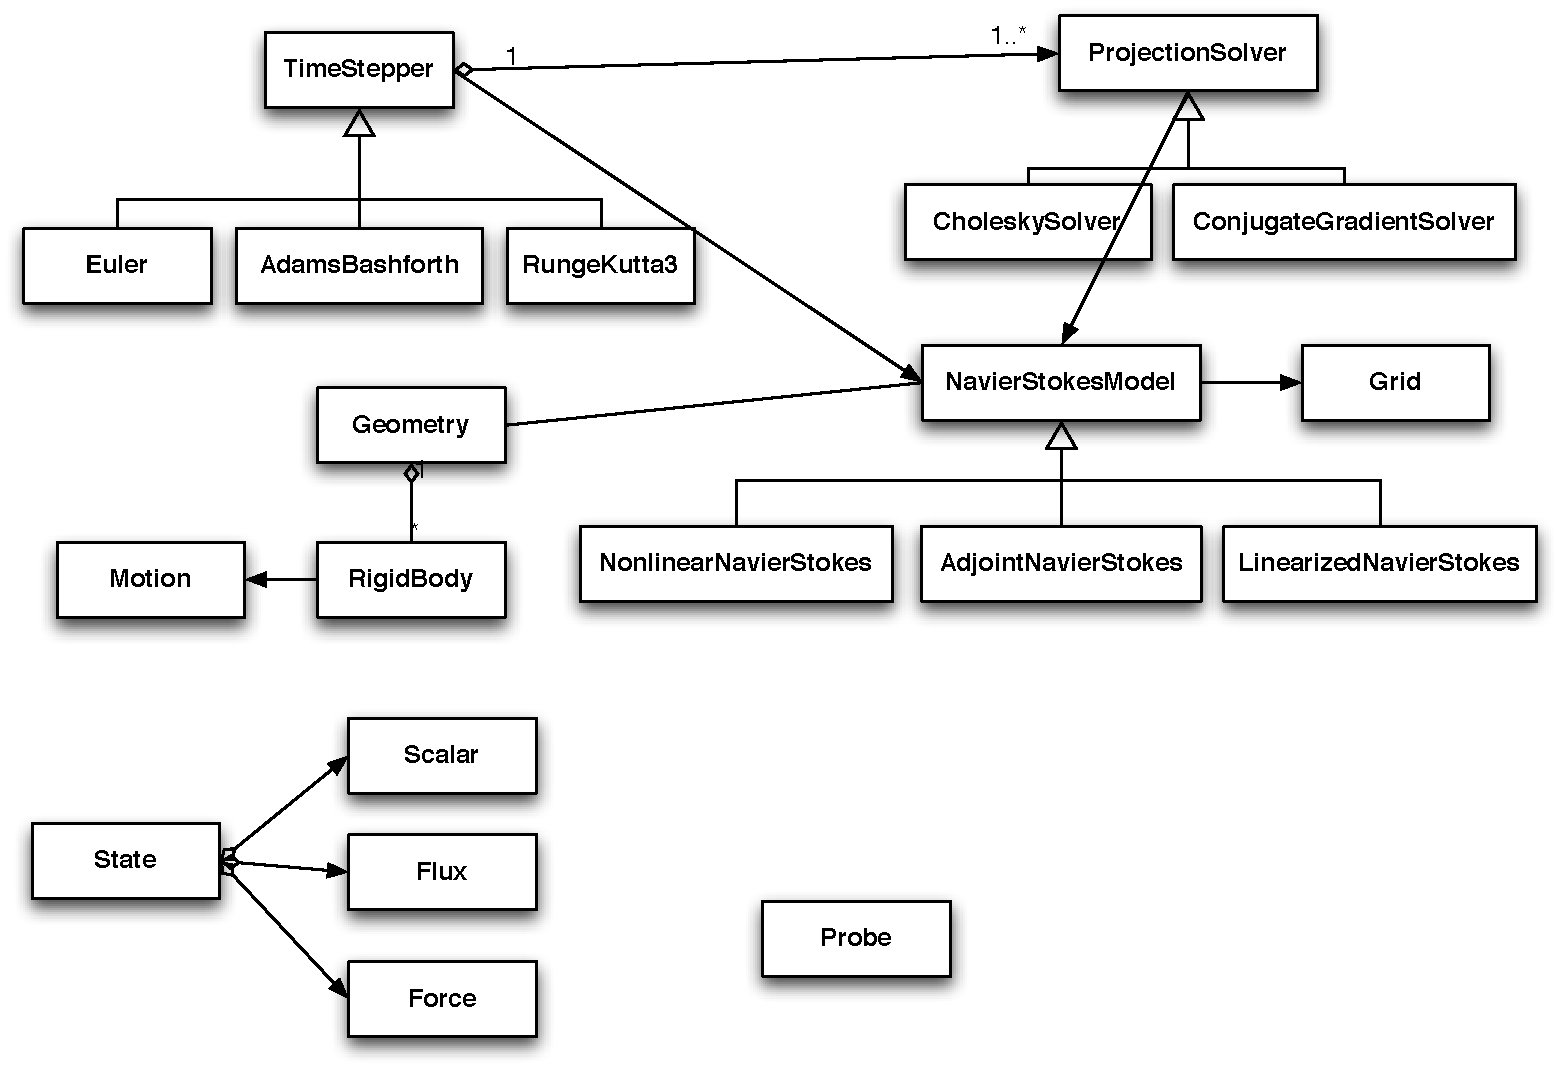
\includegraphics[width=0.95\linewidth]{IBFSDesign}
\caption{Diagram of classes and their collaborations.}
\label{fig:class_diagram}
\end{figure}

\subsection{TimeStepper}
Abstract base class to advance a flow field forward in time.

The governing equations are in the form
\begin{equation}
\begin{aligned}
\frac{d\gamma}{dt} + Bf &= L\gamma + N(q)\\
C\gamma &= b
\end{aligned}
\label{eq:model}
\end{equation}
where the operators in these equations are defined in the associated instance of \class{NavierStokesModel}.  Note that the nonlinear term depends only on the fluxes~$q$, but the fluxes can be computed from the circulation~$\gamma$ by~(\ref{eq:compute_psi}--\ref{eq:compute_q}).

A \class{TimeStepper} instance has a method \fn{advance} that takes a \class{State}, and computes the value at the next timestep, overwriting the values passed in.  The instance has a pointer to a model (of type \class{NavierStokesModel}), which contains information about the \class{Grid} and \class{Geometry}, as well as the equations to be solved (e.g., \class{LinearNavierStokes}, \class{AdjointNavierStokes}), and instantiates its own \class{ProjectionSolver} as appropriate, for solving the projection step of the equations.  For instance, for a stationary body, the \class{CholeskySolver} should be used, and for moving bodies, for which the projection step in (\ref{eq:projection_alg}) varies at each timestep, an iterative solver such as the \class{ConjugateGradientSolver} is needed.

Note that \class{TimeStepper} is an abstract class, and cannot be instantiated directly.  One of its subclasses must be instantiated.

\paragraph{Interactions}
A \class{TimeStepper} object creates an appropriate \class{ProjectionSolver} object, which it uses for solving the projection step.  The terms $L$, $B$, $C$, and $N(x)$ are provided by a \class{NavierStokesSolver}.  The quantities to be stepped forward are contained in a \class{State}.

\paragraph{Interface}
\begin{description}
	\item \fn{TimeStepper}(NavierStokesModel model, double timestep)\\
		Constructor.  Setup all routines necessary to use \virtualfn{advance}, to step the solution forward by the given timestep.  Note that creation of the \class{ProjectionSolver} should be deferred to the subclasses, but determination of which type of solver to instantiate should be handled by the base class.  (Use Abstract Factory or Factory Method design pattern?)
	\item \fn{\~\null TimeStepper}()\\
		Destructor.
	\item void \virtualfn{advance}(State x)\\
	 	Advance the state x forward one step, overwriting with the new value.  Pure virtual function: subclasses must override this.
\end{description}
\paragraph{Protected}
\begin{description}
	\item ProjectionSolver\& \fn{create\_solver}(double alpha)\\
		Return a reference to a \class{ProjectionSolver} of the appropriate type (e.g., conjugate gradient or Cholesky), with the appropriate initializations, e.g. for filename or tolerance.
		
		\todo{Look up Factory Method design pattern, or what is a standard way to do this: subclasses need to be able to create different ProjectionSolvers, but should not need to mess with logic of choosing Cholesky vs Conj Gradient, specifying tolerance, filenames, etc.}
\end{description}

\paragraph{Design choices}
\todo{Discuss Abstract Factory or Factory Method design pattern, or whatever we end up using.}

\paragraph{Implementation}
The functionality of the projection step~(\ref{eq:projection_alg}) is contained in the \class{ProjectionSolver}, so the only portion derived classes need to implement when overriding \virtualfn{advance} is a description of the timestepper as in~(\ref{eq:timestepper}), followed by a call to \fn{\_solver.solve}(a,b,$\gamma^{n+1}$,$f^{n+1}$).  Note that a \class{CholeskySolver} should be instantiated when the body is stationary, while a \class{ConjugateGradientSolver} should be used when the body is moving, since the $B$ and $C$ matrices change at each step.

\subsubsection{Euler}
Timestepper using Crank-Nicolson for linear terms, Explicit Euler for nonlinear terms.

\paragraph{Interface}
\begin{description}
	\item void \fn{advance}(State x)\\
		Advance the state forward one step, overwriting with the new value.  
\end{description}

In particular, \fn{advance}$(\gamma,f)$ returns the solution of
	\begin{align}
		(1-\frac{h}{2}L)\gamma^{n+1} + hBf &= (1 + \frac{h}{2}L)\gamma^n + h N(q^n)\\
		C\gamma^{n+1} &= b_{n+1}
	\end{align}
where $h$ is the timestep.  Here, in the notation of~(\ref{eq:constrained}),
\begin{align}
	\mathcal{A} &= 1-\frac{h}{2} L\\
	\mathcal{B} &= hB\\
	\mathcal{C} &= C\\
	a &= (1+\frac{h}{2}L)\gamma^n + hN(q^n)\\
	b &= b_{n+1}
\end{align}
where quantities on the right-hand side are specified by the associated \class{NavierStokesModel}.

\subsubsection{AdamsBashforth}
Timestepper using Crank-Nicolson for linear terms, Adams Bashforth for nonlinear terms.

\paragraph{Interface}
\begin{description}
	\item void \fn{advance}(State x)\\
		Advance the state forward one step, overwriting with the new value.  If information about the previous timestep is available, use Adams-Bashforth for nonlinear terms; otherwise, use explicit Euler.
	\item void \fn{set\_previous\_state}(State x)\\
		Initialize the value of $x$ at the previous timestep.
\end{description}

In particular, \fn{advance}$(\gamma,f)$ returns the solution of
	\begin{align}
		(1-\frac{h}{2}L)\gamma^{n+1} + hBf &= (1 + \frac{h}{2}L)\gamma^n + \frac{h}{2} \big(3N(q^n) - N(q^{n-1})\big)\\
		C\gamma^{n+1} &= b_{n+1}
	\end{align}
where $h$ is the timestep.  Here, in the notation of~(\ref{eq:constrained}),
\begin{equation}
	a = (1+\frac{h}{2}L)\gamma^n + \frac{h}{2}(3N(q^n) - N(q^{n-1})
\end{equation}
with other parameters the same as \class{Euler}.

Note: storing the previous value~$N(q^{n-1})$ is the responsibility of \class{AdamsBashforth}.

\paragraph{Implementation}
Note that it is sufficient to store the nonlinear terms~$N(\gamma)$ at the previous timestep, rather than the whole state. This saves both memory and time, since the nonlinear terms need not be recomputed at the next step.

\subsubsection{RungeKutta2}
Timestepper using Crank-Nicolson for linear terms, RK2 for nonlinear terms.

Uses the scheme given by Peyret, p.~148\cite{Peyret}, for $\alpha=1$, $\beta=1/2$:
% TODO: add Peyret book to master.bib
\begin{align}
	(1 - \frac{h}{2}L)x_1 + hBf_1 &= (1+\frac{h}{2}L)x^n + hN(x^n)\\
	Cx_1 &= b_{n+1}\\
	(1-\frac{h}{2}L)x^{n+1} + hBf^{n+1} &= (1 + \frac{h}{2}L)x^n + \frac{h}{2}\big(N(x^n) + N(x_1)\big)\\
	Cx^{n+1} &= b_{n+1}
\end{align}
Note that the equations for $x_1$ correspond to an Euler-CN step.  Conveniently, both steps use the same values of $\mathcal{A}$, $\mathcal{B}$, and $\mathcal{C}$ as \class{Euler} and \class{AdamsBashforth}, so this scheme needs only one \class{ProjectionSolver}.

\subsubsection{RungeKutta3}
Timestepper using Crank-Nicolson for linear terms, 3rd-order Runge-Kutta for nonlinear.

Uses the scheme given by Peyret, p.~149\cite{Peyret}:
\begin{align}
	Q_1 &= hN(x^n)\\
	(1-\frac{h}{6}L)x_1 + \frac{h}{3}Bf_1 &= (1+\frac{h}{6}L)x^n + \frac{h}{3}Q_1\\
	Cx_1 &= b_{n+1/3}\\
	Q_2 &= -\frac{5}{9} Q_1 + hN(x_1)\\
	(1-\frac{5h}{24}L)x_2 + \frac{5h}{12}Bf_2 &= (1+\frac{5h}{24}L)x_1 + \frac{15}{16}Q_2\\
	Cx_2 &= b_{n+3/4}\\
	Q_3 &= -\frac{153}{128} Q_2 + hN(x_2)\\
	(1-\frac{h}{8}L)x^{n+1} + \frac{h}{4}Bf^{n+1} &= (1+\frac{h}{8}L)x_2 + \frac{8}{15}Q_3\\
	Cx^{n+1} &= b_{n+1}
\end{align}
In this case, we see that we have three different values for the matrices $\mathcal{A}$, $\mathcal{B}$ and $\mathcal{C}$, for the three different stages of the scheme, and three different calls to the \class{ProjectionSolver} are required.  Best to have three different instances of this solver, since in the stationary case, three different Cholesky factorizations need to be computed and stored.

\subsection{ProjectionSolver}
Solve a system of the form
\begin{equation}
\begin{aligned}
	(1 - \frac{\alpha}{2}L)x + \alpha Bf &= a\\
	Cx &= b
\end{aligned}
\label{eq:projection_specific}
\end{equation}
for $f$ and $x$, using the algorithm~(\ref{eq:projection_alg}).  Note that this form of the equations arises for all of the timesteppers considered so far.  The parameter $\alpha$ is fixed, and the operators $L$, $B$, and $C$ are determined by an associated \class{NavierStokesModel}.

This is an abstract base class, and may not be instantiated directly.

\paragraph{Collaborations}
This class is used by \class{TimeStepper}, and contains a pointer to a \class{NavierStokesModel}.

\paragraph{Interface}
\begin{description}
	\item \fn{ProjectionSolver}(NavierStokesModel model, double alpha)\\
		Constructor.  Setup all routines necessary to use \virtualfn{solve}, including the protected methods \fn{Ainv}, \fn{B}, and \fn{C}.
	\item \fn{\~\null ProjectionSolver}()\\
		Destructor.
	\item void \fn{solve}(Scalar a, Force b, Scalar gamma, Force f)\\
	 	Solve the system~(\ref{eq:projection_specific}) using the algorithm~(\ref{eq:projection_alg}.  Inputs are $a$ and $b$, and the solution is returned in $x$, $f$.
\end{description}
\paragraph{Protected methods}
\begin{description}
	\item Scalar \fn{Ainv}(Scalar x)\\
		Compute $\mathcal{A}^{-1}x=(1+(\alpha/2)L)^{-1}x$ for a projection of the form~(\ref{eq:constrained})
	\item Scalar \fn{B}(Force f)\\
		Compute $\mathcal{B}f=\alpha Bf$, for a projection of the form~(\ref{eq:constrained}).
	\item Force \fn{C}(Scalar x)\\
		Compute $\mathcal{C}x=Cx$ for a projection of the form~(\ref{eq:constrained}).
	\item Force \fn{M}(Force f)\\
		Compute $\mathcal{M}f=\mathcal{C}\mathcal{A}^{-1}\mathcal{B}f$, the matrix that must be inverted in the second step of the algorithm~(\ref{eq:projection_alg}).  Note that for the Navier-Stokes equations, this operator should be symmetric ($\mathcal{M}=\mathcal{M}^T$).
	\item Force \virtualfn{Minv}(Force b)\\
		Solve $\mathcal{M}f=b$ for $f$.  Pure virtual function: must be overloaded by subclasses.
	\item const Geometry\& \fn{get\_geometry}()\\
		Return a reference to the associated \class{Geometry}.
\end{description}

\subsubsection{CholeskySolver}
Subclass of \class{ProjectionSolver}, in which $\mathcal{M}f=b$ is solved directly.

This class assumes the matrix~$\mathcal{M}$ is symmetric, and computes the Cholesky decomposition when it is instantiated.

\paragraph{Interface}
\begin{description}
	\item \fn{CholeskySolver}(NavierStokesModel model, double alpha)\\
		Constructor.  Note that before using \fn{Minv} (needed by \fn{solve} in the base class), one must first call either \fn{compute\_cholesky} or \fn{load\_cholesky}.
	\item Force \fn{Minv}(Force b)\\
		Solve $\mathcal{M}f = b$ directly using a Cholesky factorization already computed.
	\item void \fn{compute\_cholesky}()\\
		Compute the Cholesky decomposition of~$\mathcal{M}$, storing it as private data.
	\item bool \fn{load\_cholesky}(string fileName)\\
		Load a Cholesky decomposition from the specified file.  Returns true if successful.
	\item bool \fn{save\_cholesky}(string fileName)\\
		Save a Cholesky decomposition to the specified file, overwriting if necessary.  Returns true if successful.
\end{description}

\paragraph{Design alternatives}
A different design would be for the constructor to take a filename as an argument (or deduce it from the name in the associated Geometry object), and automatically try to load the file, calling \fn{compute\_cholesky} if the file was not found, or was invalid.  However, the call to \fn{compute\_cholesky} can be time consuming, so it seems like a better design to have to explicitly call that, so the constructor does not mysteriously take a very long time.  The approach above also gives greater flexibility in using this class.

\paragraph{Implementation}
The factorization of $\mathcal{M}$ should of course be stored as private data.  One suggestion is to have a flag to check whether the factorization has been performed, and When saving and loading these factorizations, it would be good to save/load the name of the \class{Geometry} the configuration is being saved for.  This would allow a simple check whether a loaded file matches the current geometry.  Since the solver already knows about the geometry (through the \class{NavierStokesModel} instance passed to the constructor, made available through the \fn{get\_geometry} method), this name does not need to be passed explicitly to the \class{CholeskySolver}.

\subsubsection{ConjugateGradientSolver}
Subclass of \class{ProjectionSolver}, in which $\mathcal{M}f=b$ is solved iteratively, using a conjugate gradient method.

This class assumes the matrix~$\mathcal{M}$ is symmetric, and iterates until a specified tolerance has been reached.

\paragraph{Interface}
\begin{description}
	\item \fn{ConjugateGradientSolver}(NavierStokesModel model, double alpha, double tolerance)\\
		Constructor.  Store tolerance as private data.
	\item void \fn{set\_tolerance}(double tolerance)
	\item double \fn{get\_tolerance}()
	\item Force \fn{Minv}(Force b)\\
		Solve $\mathcal{M}f = b$ directly using a conjugate gradient method.
\end{description}


\subsection{NavierStokesModel}
Provide operators $L$, $B$, $C$, and $N(q)$ for a model of the form~(\ref{eq:model}).

The operators $B$, $C$, and~$N$ are specified directly, and $L$ is specified by transformations $S$ and $S^{-1}$ and a diagonal matrix $\Lambda$, such that $L=S^{-1}\Lambda S$.

This is an abstract base class, and may not be instantiated directly, but all operators are defined in the base class except for the nonlinear term~$N(q)$.  \todo{Look up how the nonlinear term should be computed, from refs in Tim's paper, or talking to Sunil.  Also look more carefully at the other operators to see whether they need boundary conditions passed as additional parameters, or what else should be included in the objects passed to them.}

\paragraph{Interface}
\begin{description}
	\item \fn{NavierStokesModel}(Grid grid, Geometry\& geom)\\
		Constructor.  Set up the appropriate data needed to evaluate $\Lambda$, and the discrete sin transform $S$, $S^{-1}$.  Does not make a local copy of \class{Geometry}, but instead keeps a reference (or pointer) to the one passed.
	\item \fn{\~NavierStokesModel}()\\
	\item const Geometry\& \fn{get\_geometry}()\\
		Return a reference to the associated \class{Geometry}.
	\item const Grid\& \fn{get\_grid}()\\
		Return a reference to the associated \class{Grid}.
	\item const Scalar\& \fn{get\_lambda}()\\
		Return a reference to the eigenvalues $\Lambda$ of~$L$.
	\item Scalar \fn{S}(Scalar g)\\
		Transform to eigenvectors of~$L$ (discrete sin transform).
	\item Scalar \fn{Sinv}(Scalar ghat)\\
		Inverse transform $S^{-1}$.  Note that for the discrete sin transform, $S^{-1}$ should equal~$S$, but in some implementations, these may differ by a normalization constant.
	\item Scalar \fn{B}(Force f)\\
		Return $Bf$, as in~(\ref{eq:model}).
	\item Force \fn{C}(Scalar gamma)\\
		Return $C\gamma$, as in~(\ref{eq:model}).
	\item Flux \fn{regularize}(Force f) \\
		Operator $E^T$ in~(\ref{eq:navier_stokes}).
	\item Force \fn{regularize}(Flux q) \\
		Transpose of regularize, operator $E$ in~(\ref{eq:navier_stokes}).
	\item void \fn{update\_regularization}() \\
		Update the operators \fn{regularize}.  Must be called whenever the body position changes.
\end{description}
\paragraph{Protected}
\begin{description}
	\item Scalar \fn{bilinear}(State x1, State x2)\\
		Return bilinear term, used by subclasses (e.g. $N(q)=\operatorname{bilinear}(q,q)$).
\end{description}

\paragraph{Design notes}
Another option is to define \fn{regularize} in the \class{Geometry} class, so that it can be more easily updated when the body moves (then these updates occur only within one class).  However, this does not seem as appropriate, since otherwise \class{Geometry} does not need to know any information about the \class{Grid}, which is needed to compute regularization operators.  Also, all other operators are defined within the \class{NavierStokesModel}, so \fn{regularize} seems to fit better here.

\subsubsection{NonlinearNavierStokes}
Define the nonlinear term for the full nonlinear Navier-Stokes equations.
\todo{Get the explicit form of this from Sunil, from Tim's papers, or from the old code.}
\paragraph{Interface}
\begin{description}
	\item Scalar \fn{nonlinear}(State x)
\end{description}

\subsubsection{LinearNavierStokes}
Define the ``nonlinear'' term $N(q)$ for Navier-Stokes equations linearized about a base flow $x_0$.

\paragraph{Interface}
\begin{description}
	\item \fn{LinearNavierStokes}(Grid grid, Geometry geom, State baseflow)\\
		Constructor for Navier-Stokes equations linearized about a constant equilibrium solution given by baseflow.
	\item Scalar \fn{nonlinear}(State x)
\end{description}

\subsubsection{AdjointNavierStokes}
Define the ``nonlinear'' term $N(q)$ for adjoint Navier-Stokes equations, linearized about a base flow~$q_0$.  Note that, if the adjoint is defined with respect to an inner product weighted by the inverse Laplacian, then the adjoint equations differ from the linearized equations only in the nonlinear term, as described in~\cite{AhuRow-08}.

\paragraph{Interface}
\begin{description}
	\item \fn{AdjointNavierStokes}(Grid grid, Geometry geom, State baseflow)\\
		Constructor for adjoint equations for Navier-Stokes linearized about a constant equilibrium solution given by baseflow.
	\item Scalar \fn{nonlinear}(State x)
\end{description}

\subsection{Grid}
Define parameters associated with an Eulerian grid.

Use single grid for now.  Will want to extend to multiple grids, but choose to design the interface for a single grid first, so that we can iterate and refine the design before extending to multiple grids.

\paragraph{Interface}
\begin{description}
	\item Grid(int nx, int ny, double length)\\
		Constructor, given numbers of gridpoints in $x$ and $y$-directions, length in the $x$-direction.  A square grid is assumed.
	\item int \fn{get\_nx}()\\
		Return number of points in $x$-direction.
	\item int \fn{get\_ny}()\\
		Return number of points in $y$-direction.
	\item double \fn{get\_length}()\\
		Return length in $x$-direction.
	\item double \fn{get\_dx}()\\
		Return grid spacing (same in $x$- and $y$-directions).
		
\end{description}


\subsection{State}
Include time, Scalar gamma, Flux q, and Force f.  Possibly also boundary conditions?

\paragraph{Interface}
\begin{description}
	\item State(Grid grid, Geometry geom)\\
		Constructor.  Allocate memory for the associated objects (flux, circulation, and forces).
	\item \~\null State()\\
		Destructor.
\end{description}

\paragraph{Public data}
\begin{description}
	\item int timestep\\
		Timestep associated with the current value of the state (e.g. incremented by the \class{TimeStepper}).
	\item double time\\
		The time associated with the current value of the state (e.g. incremented by the \class{TimeStepper}).
	\item Scalar gamma\\
	\item Flux q\\
	\item Force f
\end{description}

\paragraph{Implementation}
No need to store the Grid and Geometry information in the state, since it is already contained in the contained data structures.

\subsection{Scalar}
Data structure and interface for storing a 2d array of scalars, located at cell centers, on multiple grids.

\paragraph{Interface}
\begin{description}
	\item Addition of two Scalars
	\item Subtraction of two Scalars
	\item Multiplication of a Scalar by a double
	\item Access individual elements with $(i,j)$ or $[i][j]$.
\end{description}

\paragraph{Implementation}
2d array.  Need to be able to take an FFT of this, so possibly best to allocate memory using an FFTW memory allocator (which ensures optimal alignment of doubles).  Use an array library such as Blitz++, TNT, or Boost?  (Governing principle: no matter what, make sure that the implementation of the arrays is independent from the interface, so the rest of the code does not need to change if the implementation is changed.)

\subsection{Flux}
Data structure and interface for storing a 2D array of fluxes, located at cell edges.

\subsection{Force}

\paragraph{Implementation}
Store as a 1d array, to facilitate solving linear systems for forces.

\subsection{Probe}
\subsection{Geometry}
Create, load, and save geometries composed of \class{RigidBody} objects.

This class is responsible for maintaining a list of bodies (each an instance of \class{RigidBody}, and for telling an associated \class{NavierStokesModel} when to update its regularization operators $E$ and $E^T$, for instance as used in~(\ref{eq:navier_stokes}).

Each geometry can be saved to or loaded from a file, and the interface should be designed so that it is easy to write a small utility program for creating and saving geometries (possibly with wrappers for Python or Matlab?).  

\paragraph{Interface}
\begin{description}
	\item \fn{Geometry}() \\
		Constructor
	\item \fn{\~\null Geometry}() \\
		Destructor
	\item void \fn{add\_body}(RigidBody body) \\
		Append the given \class{RigidBody} to the list of bodies in the current geometry, making a copy of it internally.
	\item void \fn{load}(istream in) \\
		Load a geometry from the specified input stream.  The format of the input file is as follows:
\begin{verbatim}
name My Geometry
body Flat plate
	line 0 0 1 0 50  # 50 points on a line
	center 0.25 0    # center at quarter chord
end
body Large Circle
	circle 2 3 5 100 # 100 points on a circle with radius 5, center (2,3)
					 # default center is (2,3)
end
body Airfoil
	raw naca0012.in  # Read in the raw data file
end
		\end{verbatim}
	 Whitespace at the beginnings of lines is ignored, and comments are started by \#.
	\item void \fn{set\_name}(string name) \\
		Set the name of the current geometry.
	\item void \fn{set\_model}(NavierStokesModel\& model) \\
		Set an associated \class{NavierStokesModel}.
	\item void \fn{move\_bodies}(double time) \\
		Update the position and velocities of the bodies, as specified by the associated \class{Motion}.  Also updates \fn{regularize} and \fn{regularizeT}, via the associated \class{NavierStokesModel}.
	\item int \fn{get\_num\_points}() \\
		Return the total number of points in all bodies.
	\item Force \fn{get\_points}() \\
		Return the list of coordinates for each point on each body.
	\item Force \fn{get\_velocities}() \\
		Return the list of velocities at each point on each body.		
\end{description}

\paragraph{Design notes}
An alternative is to specify the operators \fn{regularize} and \fn{regularizeT} in this class, rather than \class{NavierStokesModel}.  See the remarks in \class{NavierStokesModel} for reasons why this interface was chosen.

\paragraph{Implementation}
Internally, either \class{Geometry} or each \class{RigidBody} should maintain a list of the points after the motion has been applied.  These will be necessary for defining the regularization operators, but don't need to be publicly accessible.  Not sure where is the best place to keep this information.

\subsubsection{RigidBody}
Specify coordinates and center of a rigid body, and its motion in time.

\paragraph{Interface}
\begin{description}
	\item \fn{RigidBody}() \\
		Constructor.  Initialize the center to $(0,0)$.
	\item void \fn{add\_point}(double x, double y) \\
		Add the specified point to the list of points on the body's boundary.
	\item void \fn{add\_circle}(double xc, double yc, double radius, int numPoints) \\
		Add a circle with center $(x_c,y_c)$ and the given radius, with the specified number of points.
	\item void \fn{add\_line}(double x1, double y1, double x2, double y2, int numPoints) \\
		Add a line connecting $(x_1,y_1)$ and $(x_2,y_2)$, with the specified number of points.
	\item void \fn{load}(istream in) \\
		Load a list of commands from the specified input stream.  See below for file format.
	\item void \fn{load\_raw}(istream in) \\
		Load a list of points, in ASCII format, with one point per line.  Assumes the center is 
	\item void \fn{save\_raw}(ostream out) \\
		Save a list of points to a file with the specified name, overwriting if already present.
	\item int \fn{get\_num\_points}() \\
		Return the number of points on the body's boundary.
	\item bool \fn{is\_stationary}() \\
		Return true if the body is not moving in time.
	\item void \fn{set\_motion}(Motion motion) \\
		Set the evolution of the of the current body (which may be stationary or not).
	\item void \fn{set\_center}(double x, double y) \\
		Set the center of the body, about which rotations are defined.
	\item void \fn{get\_center}(double\& x, double\& y)\\
		Get the center of the body, about which rotations are defined.
	\item void \fn{set\_name} \\
		Set the name of the body
	\item string \fn{get\_name}() \\
		Return the name of the body
	\item 
\end{description}

\paragraph{File format}
Need to determine a good file format for loading/saving bodies.  ASCII is probably best, in some format easily readable by both humans and machines.  Example file format:
\begin{verbatim}
name some object
center x y
point x y
point x y
point x y
line x1 y1 x2 y2 npts
circle xc yc radius npts
raw naca0012.dat
end
\end{verbatim}
Commands should be read until the end of file is reached, or until {\tt end} is read (so that a single Geometry file can contain multiple bodies).

These commands easily map to the methods in the \class{RigidBody} interface, and are much more readable by humans than a raw list of points.  Could easily write a utility for parsing this and converting to a list of points for plotting with Matlab, Tecplot, etc.  This format contains more information than a list of points, since it says something about the structure/connectivity.

\paragraph{Implementation}
Note that if saving to a file, need to save the information in the RigidBody with more structure, e.g. specifying Point, Line, Circle objects.  Probably best to implement more simply first, just as a raw list of points, and then make more complex if needed.

\subsubsection{Motion}
Specify a position and orientation as a function of time.

Abstract base class, must be subclassed to be instantiated.

\paragraph{Interface}
\begin{description}
	\item Motion() \\
		Constructor.
	\item virtual bool \fn{is\_stationary}() \\
		Return false.  (Can be overridden by subclasses.)
	\item Euclidean2D \virtualfn{get\_position}(double time) \\
		Return a Euclidean transformation at the specified time
\end{description}

\paragraph{Design notes}
\fn{is\_stationary} returns False by default, since presumably the only subclass that would return true is \class{FixedPosition}.  Would probably be better style to make this a pure virtual function, but this way saves a little effort when making subclasses.

\subsubsection{FixedPosition}
Subclass of \class{Motion}, for a stationary body.

\paragraph{Interface}
\begin{description}
	\item FixedPosition(double x, double y, double theta) \\
		Define a \class{Motion} corresponding to a fixed position, rotation about the center.
	\item bool \fn{is\_stationary}()\\
		Return true.
\end{description}
	

\subsubsection{Euclidean2D}
Perform translations and rotations in 2D, corresponding to the action of the group $SE(2)$.

\paragraph{Interface}
\begin{description}
	\item Euclidean2D(double x, double y, double theta)
		Constructor for a transformation corresponding to rotation by $\theta$, followed by translation by $(x,y)$.
	\item set\_velocity(double xdot, double ydot, double thetadot) \\
		Set the tangent vector, for use in \fn{mapVelocity}
	\item map\_position(double a,double b, double\& a\_new, double\& b\_new)\\
		Given the point $(a,b)$, compute the mapped point $(a\_\text{new},b\_\text{new})$.
	\item map\_velocity(double u, double v, double\& u\_new, double\& v\_new)\\
		Given the velocity $(u,v)$, compute the mapped velocity $(u_\text{new},v_\text{new})$.  If velocity of the mapping has not been set, assume zero velocity $\dot x = \dot y = 0$.
\end{description}

\bibliographystyle{abbrv}
\bibliography{jabbrv,master}

% \begin{thebibliography}{1}
% 
% \bibitem{ColTai-07}
% T.~Colonius and K.~Taira.
% \newblock A fast immersed boundary method using a nullspace approach and
%   multi-domain far-field boundary conditions.
% \newblock {\em Comp.\ Meth.\ Appl.\ Mech.\ Eng.}, 197(25-28):2131--46, 2008.
% 
% \end{thebibliography}

\end{document}
